\documentclass{standalone}
\usepackage{tikz}
\usetikzlibrary{patterns}
\usetikzlibrary{positioning}
\usetikzlibrary{patterns, positioning}
\usetikzlibrary{shapes.misc}
\usepackage[outline]{contour}
\contourlength{1.5pt} 
\usetikzlibrary{calc}
        \usepackage{relsize}
        \tikzset{fontscale/.style = {font=\relsize{#1}}}

\begin{document}
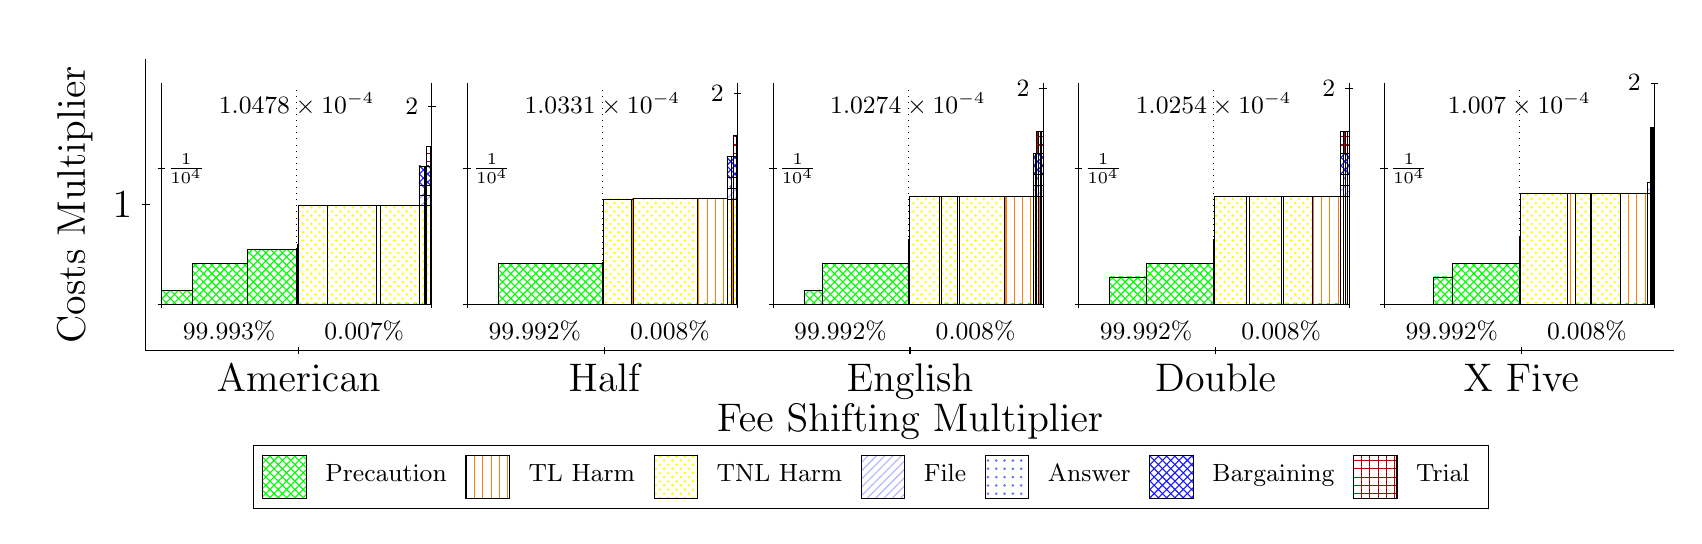
\begin{tikzpicture}
\clip(-0.5,-1.1) rectangle +(20.91,6.2);
\draw[black] (1,1) -- (1,4.7);
\node[rotate=90, fontscale=2, anchor=center] at (0.1, 2.85) {Costs Multiplier};
\draw[black] (0.95,2.85) -- (1.05,2.85);
\node[fontscale=2, anchor=east] at (0.95, 2.85) {1};

\draw[black] (1,1) -- (20.41,1);
\node[fontscale=2, anchor=center] at (10.705, 0.1) {Fee Shifting Multiplier};
\draw[black] (2.941,0.95) -- (2.941,1.05);
\node[fontscale=2, anchor=north] at (2.941, 0.95) {American};
\draw[black] (6.823,0.95) -- (6.823,1.05);
\node[fontscale=2, anchor=north] at (6.823, 0.95) {Half};
\draw[black] (10.705,0.95) -- (10.705,1.05);
\node[fontscale=2, anchor=north] at (10.705, 0.95) {English};
\draw[black] (14.587,0.95) -- (14.587,1.05);
\node[fontscale=2, anchor=north] at (14.587, 0.95) {Double};
\draw[black] (18.469,0.95) -- (18.469,1.05);
\node[fontscale=2, anchor=north] at (18.469, 0.95) {X Five};


\draw[pattern=crosshatch, pattern color=green,draw=black,very thin] (1.2,1.592) rectangle (1.5947,1.764);
\draw[pattern=crosshatch, pattern color=green,draw=black,very thin] (1.5947,1.592) rectangle (2.2894,2.1081);
\draw[pattern=crosshatch, pattern color=green,draw=black,very thin] (2.2894,1.592) rectangle (2.916,2.2802);
\draw[pattern=crosshatch, pattern color=green,draw=black,very thin] (2.916,1.592) rectangle (2.9243,1.592);
\draw[pattern=north east lines, pattern color=blue!30,draw=black,very thin] (2.916,1.592) rectangle (2.9243,1.7172);
\draw[pattern=dots,  pattern color=blue!60,draw=black,very thin] (2.916,1.7172) rectangle (2.9243,1.8425);
\draw[pattern=crosshatch,      pattern color=blue!90,draw=black,very thin] (2.916,1.8425) rectangle (2.9243,2.0929);
\draw[pattern=crosshatch, pattern color=green,draw=black,very thin] (2.9243,1.592) rectangle (2.9274,1.592);
\draw[pattern=north east lines, pattern color=blue!30,draw=black,very thin] (2.9243,1.592) rectangle (2.9274,1.7173);
\draw[pattern=dots,  pattern color=blue!60,draw=black,very thin] (2.9243,1.7173) rectangle (2.9274,1.8425);
\draw[pattern=crosshatch,      pattern color=blue!90,draw=black,very thin] (2.9243,1.8425) rectangle (2.9274,2.093);
\draw[pattern=crosshatch, pattern color=green,draw=black,very thin] (2.9274,1.592) rectangle (2.9334,1.592);
\draw[pattern=north east lines, pattern color=blue!30,draw=black,very thin] (2.9274,1.592) rectangle (2.9334,1.7172);
\draw[pattern=dots,  pattern color=blue!60,draw=black,very thin] (2.9274,1.7172) rectangle (2.9334,1.8425);
\draw[pattern=crosshatch,      pattern color=blue!90,draw=black,very thin] (2.9274,1.8425) rectangle (2.9334,2.0929);
\draw[pattern=grid,            pattern color=red!70!black,draw=black,very thin] (2.9274,2.0929) rectangle (2.9334,2.3434);
\draw[pattern=crosshatch, pattern color=green,draw=black,very thin] (2.9334,1.592) rectangle (2.9354,1.592);
\draw[pattern=north east lines, pattern color=blue!30,draw=black,very thin] (2.9334,1.592) rectangle (2.9354,1.7173);
\draw[pattern=dots,  pattern color=blue!60,draw=black,very thin] (2.9334,1.7173) rectangle (2.9354,1.8425);
\draw[pattern=crosshatch,      pattern color=blue!90,draw=black,very thin] (2.9334,1.8425) rectangle (2.9354,2.093);
\draw[pattern=grid,            pattern color=red!70!black,draw=black,very thin] (2.9334,2.093) rectangle (2.9354,2.3434);
\draw[pattern=crosshatch, pattern color=green,draw=black,very thin] (2.9354,1.592) rectangle (3.3039,1.592);
\draw[pattern=crosshatch dots, pattern color=yellow,draw=black,very thin] (2.9354,1.592) rectangle (3.3039,2.8443);
\draw[pattern=crosshatch, pattern color=green,draw=black,very thin] (3.3039,1.592) rectangle (3.3061,1.592);
\draw[pattern=vertical lines, pattern color=orange,draw=black,very thin] (3.3039,1.592) rectangle (3.3061,2.8443);
\draw[pattern=crosshatch, pattern color=green,draw=black,very thin] (3.3061,1.592) rectangle (3.9318,1.592);
\draw[pattern=crosshatch dots, pattern color=yellow,draw=black,very thin] (3.3061,1.592) rectangle (3.9318,2.8443);
\draw[pattern=crosshatch, pattern color=green,draw=black,very thin] (3.9318,1.592) rectangle (3.977,1.592);
\draw[pattern=vertical lines, pattern color=orange,draw=black,very thin] (3.9318,1.592) rectangle (3.977,2.8443);
\draw[pattern=crosshatch, pattern color=green,draw=black,very thin] (3.977,1.592) rectangle (4.4677,1.5921);
\draw[pattern=crosshatch dots, pattern color=yellow,draw=black,very thin] (3.977,1.5921) rectangle (4.4677,2.8443);
\draw[pattern=crosshatch, pattern color=green,draw=black,very thin] (4.4677,1.592) rectangle (4.5339,1.592);
\draw[pattern=crosshatch dots, pattern color=yellow,draw=black,very thin] (4.4677,1.592) rectangle (4.5339,2.8443);
\draw[pattern=north east lines, pattern color=blue!30,draw=black,very thin] (4.4677,2.8443) rectangle (4.5339,2.9695);
\draw[pattern=dots,  pattern color=blue!60,draw=black,very thin] (4.4677,2.9695) rectangle (4.5339,3.0948);
\draw[pattern=crosshatch,      pattern color=blue!90,draw=black,very thin] (4.4677,3.0948) rectangle (4.5339,3.3452);
\draw[pattern=crosshatch, pattern color=green,draw=black,very thin] (4.5339,1.592) rectangle (4.5435,1.592);
\draw[pattern=vertical lines, pattern color=orange,draw=black,very thin] (4.5339,1.592) rectangle (4.5435,2.8443);
\draw[pattern=north east lines, pattern color=blue!30,draw=black,very thin] (4.5339,2.8443) rectangle (4.5435,2.9695);
\draw[pattern=dots,  pattern color=blue!60,draw=black,very thin] (4.5339,2.9695) rectangle (4.5435,3.0948);
\draw[pattern=crosshatch,      pattern color=blue!90,draw=black,very thin] (4.5339,3.0948) rectangle (4.5435,3.3452);
\draw[pattern=crosshatch, pattern color=green,draw=black,very thin] (4.5435,1.592) rectangle (4.5503,1.592);
\draw[pattern=crosshatch dots, pattern color=yellow,draw=black,very thin] (4.5435,1.592) rectangle (4.5503,2.8443);
\draw[pattern=north east lines, pattern color=blue!30,draw=black,very thin] (4.5435,2.8443) rectangle (4.5503,2.9695);
\draw[pattern=dots,  pattern color=blue!60,draw=black,very thin] (4.5435,2.9695) rectangle (4.5503,3.0948);
\draw[pattern=crosshatch,      pattern color=blue!90,draw=black,very thin] (4.5435,3.0948) rectangle (4.5503,3.3452);
\draw[pattern=crosshatch, pattern color=green,draw=black,very thin] (4.5503,1.592) rectangle (4.5634,1.592);
\draw[pattern=vertical lines, pattern color=orange,draw=black,very thin] (4.5503,1.592) rectangle (4.5634,2.8443);
\draw[pattern=north east lines, pattern color=blue!30,draw=black,very thin] (4.5503,2.8443) rectangle (4.5634,2.9695);
\draw[pattern=dots,  pattern color=blue!60,draw=black,very thin] (4.5503,2.9695) rectangle (4.5634,3.0948);
\draw[pattern=crosshatch,      pattern color=blue!90,draw=black,very thin] (4.5503,3.0948) rectangle (4.5634,3.3452);
\draw[pattern=crosshatch, pattern color=green,draw=black,very thin] (4.5634,1.592) rectangle (4.612,1.592);
\draw[pattern=crosshatch dots, pattern color=yellow,draw=black,very thin] (4.5634,1.592) rectangle (4.612,2.8443);
\draw[pattern=north east lines, pattern color=blue!30,draw=black,very thin] (4.5634,2.8443) rectangle (4.612,2.9695);
\draw[pattern=dots,  pattern color=blue!60,draw=black,very thin] (4.5634,2.9695) rectangle (4.612,3.0948);
\draw[pattern=crosshatch,      pattern color=blue!90,draw=black,very thin] (4.5634,3.0948) rectangle (4.612,3.3452);
\draw[pattern=grid,            pattern color=red!70!black,draw=black,very thin] (4.5634,3.3452) rectangle (4.612,3.5957);
\draw[pattern=crosshatch, pattern color=green,draw=black,very thin] (4.612,1.592) rectangle (4.6185,1.592);
\draw[pattern=vertical lines, pattern color=orange,draw=black,very thin] (4.612,1.592) rectangle (4.6185,2.8443);
\draw[pattern=north east lines, pattern color=blue!30,draw=black,very thin] (4.612,2.8443) rectangle (4.6185,2.9695);
\draw[pattern=dots,  pattern color=blue!60,draw=black,very thin] (4.612,2.9695) rectangle (4.6185,3.0948);
\draw[pattern=crosshatch,      pattern color=blue!90,draw=black,very thin] (4.612,3.0948) rectangle (4.6185,3.3452);
\draw[pattern=grid,            pattern color=red!70!black,draw=black,very thin] (4.612,3.3452) rectangle (4.6185,3.5957);
\draw[pattern=crosshatch, pattern color=green,draw=black,very thin] (4.6185,1.592) rectangle (4.6264,1.592);
\draw[pattern=crosshatch dots, pattern color=yellow,draw=black,very thin] (4.6185,1.592) rectangle (4.6264,2.8443);
\draw[pattern=north east lines, pattern color=blue!30,draw=black,very thin] (4.6185,2.8443) rectangle (4.6264,2.9695);
\draw[pattern=dots,  pattern color=blue!60,draw=black,very thin] (4.6185,2.9695) rectangle (4.6264,3.0948);
\draw[pattern=crosshatch,      pattern color=blue!90,draw=black,very thin] (4.6185,3.0948) rectangle (4.6264,3.3452);
\draw[pattern=grid,            pattern color=red!70!black,draw=black,very thin] (4.6185,3.3452) rectangle (4.6264,3.5957);
\draw[pattern=crosshatch, pattern color=green,draw=black,very thin] (4.6264,1.592) rectangle (4.632,1.592);
\draw[pattern=vertical lines, pattern color=orange,draw=black,very thin] (4.6264,1.592) rectangle (4.632,2.8443);
\draw[pattern=north east lines, pattern color=blue!30,draw=black,very thin] (4.6264,2.8443) rectangle (4.632,2.9695);
\draw[pattern=dots,  pattern color=blue!60,draw=black,very thin] (4.6264,2.9695) rectangle (4.632,3.0948);
\draw[pattern=crosshatch,      pattern color=blue!90,draw=black,very thin] (4.6264,3.0948) rectangle (4.632,3.3452);
\draw[pattern=grid,            pattern color=red!70!black,draw=black,very thin] (4.6264,3.3452) rectangle (4.632,3.5957);
\node[font=\small,text=black,anchor=north] at (2.916, 4.4) {$1.0478\times 10^{-4}$};
\draw[black,very thin] (1.2,1.592) -- (1.2,4.4);
\draw[black,very thin] (1.15,1.592) -- (1.25,1.592);
\node[font=\small,text=black, anchor=west] at (1.15, 1.592) {};
\draw[black,very thin] (1.15,3.3124) -- (1.25,3.3124);
\node[font=\small,text=black, anchor=west] at (1.15, 3.3124) {$\frac{1}{10^{4}}$};

\draw[black,dotted,very thin] (2.916,1.6762) -- (2.916,4.3158);
\draw[black,very thin] (4.632,1.592) -- (4.632,4.4);
\draw[black,very thin] (4.582,4.0966) -- (4.682,4.0966);
\node[font=\small,text=black, anchor=east] at (4.582, 4.0966) {\contour{white}{2}};

\draw[black,very thin] (1.2,1.592) -- (4.632,1.592);
\draw[black,very thin] (1.2,1.542) -- (1.2,1.642);
\node[font=\small,text=black, anchor=north] at (1.2, 1.542) {};
\draw[black,very thin] (4.632,1.542) -- (4.632,1.642);
\node[font=\small,text=black, anchor=north] at (4.632, 1.542) {};

\node[font=\small,text=black,anchor=south] at (2.058, 0.992) {99.993\%};
\node[font=\small,text=black,anchor=south] at (3.774, 0.992) {0.007\%};

\draw[pattern=crosshatch, pattern color=green,draw=black,very thin] (5.4767,1.592) rectangle (6.798,2.1081);
\draw[pattern=north east lines, pattern color=blue!30,draw=black,very thin] (6.798,1.592) rectangle (6.8058,1.7255);
\draw[pattern=dots,  pattern color=blue!60,draw=black,very thin] (6.798,1.7255) rectangle (6.8058,1.859);
\draw[pattern=crosshatch,      pattern color=blue!90,draw=black,very thin] (6.798,1.859) rectangle (6.8058,2.126);
\draw[pattern=north east lines, pattern color=blue!30,draw=black,very thin] (6.8058,1.592) rectangle (6.8114,1.7255);
\draw[pattern=dots,  pattern color=blue!60,draw=black,very thin] (6.8058,1.7255) rectangle (6.8114,1.859);
\draw[pattern=crosshatch,      pattern color=blue!90,draw=black,very thin] (6.8058,1.859) rectangle (6.8114,2.126);
\draw[pattern=grid,            pattern color=red!70!black,draw=black,very thin] (6.8058,2.126) rectangle (6.8114,2.393);
\draw[pattern=crosshatch dots, pattern color=yellow,draw=black,very thin] (6.8114,1.592) rectangle (7.1695,2.9269);
\draw[pattern=vertical lines, pattern color=orange,draw=black,very thin] (7.1695,1.592) rectangle (7.1858,2.9269);
\draw[pattern=crosshatch, pattern color=green,draw=black,very thin] (7.1858,1.592) rectangle (7.9985,1.592);
\draw[pattern=crosshatch dots, pattern color=yellow,draw=black,very thin] (7.1858,1.592) rectangle (7.9985,2.927);
\draw[pattern=crosshatch, pattern color=green,draw=black,very thin] (7.9985,1.592) rectangle (8.3796,1.592);
\draw[pattern=vertical lines, pattern color=orange,draw=black,very thin] (7.9985,1.592) rectangle (8.3796,2.927);
\draw[pattern=crosshatch dots, pattern color=yellow,draw=black,very thin] (8.3796,1.592) rectangle (8.4293,2.9269);
\draw[pattern=north east lines, pattern color=blue!30,draw=black,very thin] (8.3796,2.9269) rectangle (8.4293,3.0604);
\draw[pattern=dots,  pattern color=blue!60,draw=black,very thin] (8.3796,3.0604) rectangle (8.4293,3.1939);
\draw[pattern=crosshatch,      pattern color=blue!90,draw=black,very thin] (8.3796,3.1939) rectangle (8.4293,3.4609);
\draw[pattern=vertical lines, pattern color=orange,draw=black,very thin] (8.4293,1.592) rectangle (8.4576,2.9269);
\draw[pattern=north east lines, pattern color=blue!30,draw=black,very thin] (8.4293,2.9269) rectangle (8.4576,3.0604);
\draw[pattern=dots,  pattern color=blue!60,draw=black,very thin] (8.4293,3.0604) rectangle (8.4576,3.1939);
\draw[pattern=crosshatch,      pattern color=blue!90,draw=black,very thin] (8.4293,3.1939) rectangle (8.4576,3.4609);
\draw[pattern=crosshatch dots, pattern color=yellow,draw=black,very thin] (8.4576,1.592) rectangle (8.4978,2.9269);
\draw[pattern=north east lines, pattern color=blue!30,draw=black,very thin] (8.4576,2.9269) rectangle (8.4978,3.0604);
\draw[pattern=dots,  pattern color=blue!60,draw=black,very thin] (8.4576,3.0604) rectangle (8.4978,3.1939);
\draw[pattern=crosshatch,      pattern color=blue!90,draw=black,very thin] (8.4576,3.1939) rectangle (8.4978,3.4609);
\draw[pattern=grid,            pattern color=red!70!black,draw=black,very thin] (8.4576,3.4609) rectangle (8.4978,3.7279);
\draw[pattern=vertical lines, pattern color=orange,draw=black,very thin] (8.4978,1.592) rectangle (8.514,2.9269);
\draw[pattern=north east lines, pattern color=blue!30,draw=black,very thin] (8.4978,2.9269) rectangle (8.514,3.0604);
\draw[pattern=dots,  pattern color=blue!60,draw=black,very thin] (8.4978,3.0604) rectangle (8.514,3.1939);
\draw[pattern=crosshatch,      pattern color=blue!90,draw=black,very thin] (8.4978,3.1939) rectangle (8.514,3.4609);
\draw[pattern=grid,            pattern color=red!70!black,draw=black,very thin] (8.4978,3.4609) rectangle (8.514,3.7279);
\node[font=\small,text=black,anchor=north] at (6.798, 4.4) {$1.0331\times 10^{-4}$};
\draw[black,very thin] (5.082,1.592) -- (5.082,4.4);
\draw[black,very thin] (5.032,1.592) -- (5.132,1.592);
\node[font=\small,text=black, anchor=west] at (5.032, 1.592) {};
\draw[black,very thin] (5.032,3.3124) -- (5.132,3.3124);
\node[font=\small,text=black, anchor=west] at (5.032, 3.3124) {$\frac{1}{10^{4}}$};

\draw[black,dotted,very thin] (6.798,1.6762) -- (6.798,4.3158);
\draw[black,very thin] (8.514,1.592) -- (8.514,4.4);
\draw[black,very thin] (8.464,4.2619) -- (8.564,4.2619);
\node[font=\small,text=black, anchor=east] at (8.464, 4.2619) {\contour{white}{2}};

\draw[black,very thin] (5.082,1.592) -- (8.514,1.592);
\draw[black,very thin] (5.082,1.542) -- (5.082,1.642);
\node[font=\small,text=black, anchor=north] at (5.082, 1.542) {};
\draw[black,very thin] (8.514,1.542) -- (8.514,1.642);
\node[font=\small,text=black, anchor=north] at (8.514, 1.542) {};

\node[font=\small,text=black,anchor=south] at (5.94, 0.992) {99.992\%};
\node[font=\small,text=black,anchor=south] at (7.656, 0.992) {0.008\%};

\draw[pattern=crosshatch, pattern color=green,draw=black,very thin] (9.3587,1.592) rectangle (9.5905,1.764);
\draw[pattern=crosshatch, pattern color=green,draw=black,very thin] (9.5905,1.592) rectangle (10.68,2.1081);
\draw[pattern=north east lines, pattern color=blue!30,draw=black,very thin] (10.68,1.592) rectangle (10.684,1.7288);
\draw[pattern=dots,  pattern color=blue!60,draw=black,very thin] (10.68,1.7288) rectangle (10.684,1.8657);
\draw[pattern=crosshatch,      pattern color=blue!90,draw=black,very thin] (10.68,1.8657) rectangle (10.684,2.1393);
\draw[pattern=north east lines, pattern color=blue!30,draw=black,very thin] (10.684,1.592) rectangle (10.689,1.7288);
\draw[pattern=dots,  pattern color=blue!60,draw=black,very thin] (10.684,1.7288) rectangle (10.689,1.8657);
\draw[pattern=crosshatch,      pattern color=blue!90,draw=black,very thin] (10.684,1.8657) rectangle (10.689,2.1393);
\draw[pattern=grid,            pattern color=red!70!black,draw=black,very thin] (10.684,2.1393) rectangle (10.689,2.413);
\draw[pattern=crosshatch, pattern color=green,draw=black,very thin] (10.689,1.592) rectangle (10.693,1.592);
\draw[pattern=north east lines, pattern color=blue!30,draw=black,very thin] (10.689,1.592) rectangle (10.693,1.7288);
\draw[pattern=dots,  pattern color=blue!60,draw=black,very thin] (10.689,1.7288) rectangle (10.693,1.8657);
\draw[pattern=crosshatch,      pattern color=blue!90,draw=black,very thin] (10.689,1.8657) rectangle (10.693,2.1393);
\draw[pattern=grid,            pattern color=red!70!black,draw=black,very thin] (10.689,2.1393) rectangle (10.693,2.413);
\draw[pattern=crosshatch dots, pattern color=yellow,draw=black,very thin] (10.693,1.592) rectangle (11.075,2.9603);
\draw[pattern=vertical lines, pattern color=orange,draw=black,very thin] (11.075,1.592) rectangle (11.099,2.9603);
\draw[pattern=crosshatch, pattern color=green,draw=black,very thin] (11.099,1.592) rectangle (11.309,1.592);
\draw[pattern=crosshatch dots, pattern color=yellow,draw=black,very thin] (11.099,1.592) rectangle (11.309,2.9603);
\draw[pattern=crosshatch, pattern color=green,draw=black,very thin] (11.309,1.592) rectangle (11.331,1.592);
\draw[pattern=vertical lines, pattern color=orange,draw=black,very thin] (11.309,1.592) rectangle (11.331,2.9603);
\draw[pattern=crosshatch, pattern color=green,draw=black,very thin] (11.331,1.592) rectangle (11.903,1.592);
\draw[pattern=crosshatch dots, pattern color=yellow,draw=black,very thin] (11.331,1.592) rectangle (11.903,2.9603);
\draw[pattern=crosshatch, pattern color=green,draw=black,very thin] (11.903,1.592) rectangle (12.272,1.592);
\draw[pattern=vertical lines, pattern color=orange,draw=black,very thin] (11.903,1.592) rectangle (12.272,2.9603);
\draw[pattern=crosshatch dots, pattern color=yellow,draw=black,very thin] (12.272,1.592) rectangle (12.297,2.9603);
\draw[pattern=north east lines, pattern color=blue!30,draw=black,very thin] (12.272,2.9603) rectangle (12.297,3.0971);
\draw[pattern=dots,  pattern color=blue!60,draw=black,very thin] (12.272,3.0971) rectangle (12.297,3.2339);
\draw[pattern=crosshatch,      pattern color=blue!90,draw=black,very thin] (12.272,3.2339) rectangle (12.297,3.5076);
\draw[pattern=vertical lines, pattern color=orange,draw=black,very thin] (12.297,1.592) rectangle (12.312,2.9603);
\draw[pattern=north east lines, pattern color=blue!30,draw=black,very thin] (12.297,2.9603) rectangle (12.312,3.0971);
\draw[pattern=dots,  pattern color=blue!60,draw=black,very thin] (12.297,3.0971) rectangle (12.312,3.2339);
\draw[pattern=crosshatch,      pattern color=blue!90,draw=black,very thin] (12.297,3.2339) rectangle (12.312,3.5076);
\draw[pattern=crosshatch dots, pattern color=yellow,draw=black,very thin] (12.312,1.592) rectangle (12.34,2.9603);
\draw[pattern=north east lines, pattern color=blue!30,draw=black,very thin] (12.312,2.9603) rectangle (12.34,3.0971);
\draw[pattern=dots,  pattern color=blue!60,draw=black,very thin] (12.312,3.0971) rectangle (12.34,3.2339);
\draw[pattern=crosshatch,      pattern color=blue!90,draw=black,very thin] (12.312,3.2339) rectangle (12.34,3.5076);
\draw[pattern=grid,            pattern color=red!70!black,draw=black,very thin] (12.312,3.5076) rectangle (12.34,3.7812);
\draw[pattern=vertical lines, pattern color=orange,draw=black,very thin] (12.34,1.592) rectangle (12.361,2.9603);
\draw[pattern=north east lines, pattern color=blue!30,draw=black,very thin] (12.34,2.9603) rectangle (12.361,3.0971);
\draw[pattern=dots,  pattern color=blue!60,draw=black,very thin] (12.34,3.0971) rectangle (12.361,3.2339);
\draw[pattern=crosshatch,      pattern color=blue!90,draw=black,very thin] (12.34,3.2339) rectangle (12.361,3.5076);
\draw[pattern=grid,            pattern color=red!70!black,draw=black,very thin] (12.34,3.5076) rectangle (12.361,3.7812);
\draw[pattern=crosshatch, pattern color=green,draw=black,very thin] (12.361,1.592) rectangle (12.375,1.592);
\draw[pattern=crosshatch dots, pattern color=yellow,draw=black,very thin] (12.361,1.592) rectangle (12.375,2.9603);
\draw[pattern=north east lines, pattern color=blue!30,draw=black,very thin] (12.361,2.9603) rectangle (12.375,3.0971);
\draw[pattern=dots,  pattern color=blue!60,draw=black,very thin] (12.361,3.0971) rectangle (12.375,3.2339);
\draw[pattern=crosshatch,      pattern color=blue!90,draw=black,very thin] (12.361,3.2339) rectangle (12.375,3.5076);
\draw[pattern=grid,            pattern color=red!70!black,draw=black,very thin] (12.361,3.5076) rectangle (12.375,3.7812);
\draw[pattern=crosshatch, pattern color=green,draw=black,very thin] (12.375,1.592) rectangle (12.396,1.592);
\draw[pattern=vertical lines, pattern color=orange,draw=black,very thin] (12.375,1.592) rectangle (12.396,2.9603);
\draw[pattern=north east lines, pattern color=blue!30,draw=black,very thin] (12.375,2.9603) rectangle (12.396,3.0971);
\draw[pattern=dots,  pattern color=blue!60,draw=black,very thin] (12.375,3.0971) rectangle (12.396,3.2339);
\draw[pattern=crosshatch,      pattern color=blue!90,draw=black,very thin] (12.375,3.2339) rectangle (12.396,3.5076);
\draw[pattern=grid,            pattern color=red!70!black,draw=black,very thin] (12.375,3.5076) rectangle (12.396,3.7812);
\node[font=\small,text=black,anchor=north] at (10.68, 4.4) {$1.0274\times 10^{-4}$};
\draw[black,very thin] (8.964,1.592) -- (8.964,4.4);
\draw[black,very thin] (8.914,1.592) -- (9.014,1.592);
\node[font=\small,text=black, anchor=west] at (8.914, 1.592) {};
\draw[black,very thin] (8.914,3.3124) -- (9.014,3.3124);
\node[font=\small,text=black, anchor=west] at (8.914, 3.3124) {$\frac{1}{10^{4}}$};

\draw[black,dotted,very thin] (10.68,1.6762) -- (10.68,4.3158);
\draw[black,very thin] (12.396,1.592) -- (12.396,4.4);
\draw[black,very thin] (12.346,4.3285) -- (12.446,4.3285);
\node[font=\small,text=black, anchor=east] at (12.346, 4.3285) {\contour{white}{2}};

\draw[black,very thin] (8.964,1.592) -- (12.396,1.592);
\draw[black,very thin] (8.964,1.542) -- (8.964,1.642);
\node[font=\small,text=black, anchor=north] at (8.964, 1.542) {};
\draw[black,very thin] (12.396,1.542) -- (12.396,1.642);
\node[font=\small,text=black, anchor=north] at (12.396, 1.542) {};

\node[font=\small,text=black,anchor=south] at (9.822, 0.992) {99.992\%};
\node[font=\small,text=black,anchor=south] at (11.538, 0.992) {0.008\%};

\draw[pattern=crosshatch, pattern color=green,draw=black,very thin] (13.241,1.592) rectangle (13.704,1.9361);
\draw[pattern=crosshatch, pattern color=green,draw=black,very thin] (13.704,1.592) rectangle (14.562,2.1081);
\draw[pattern=north east lines, pattern color=blue!30,draw=black,very thin] (14.562,1.592) rectangle (14.568,1.7287);
\draw[pattern=dots,  pattern color=blue!60,draw=black,very thin] (14.562,1.7287) rectangle (14.568,1.8654);
\draw[pattern=crosshatch,      pattern color=blue!90,draw=black,very thin] (14.562,1.8654) rectangle (14.568,2.1389);
\draw[pattern=grid,            pattern color=red!70!black,draw=black,very thin] (14.562,2.1389) rectangle (14.568,2.4123);
\draw[pattern=crosshatch, pattern color=green,draw=black,very thin] (14.568,1.592) rectangle (14.574,1.592);
\draw[pattern=north east lines, pattern color=blue!30,draw=black,very thin] (14.568,1.592) rectangle (14.574,1.7287);
\draw[pattern=dots,  pattern color=blue!60,draw=black,very thin] (14.568,1.7287) rectangle (14.574,1.8655);
\draw[pattern=crosshatch,      pattern color=blue!90,draw=black,very thin] (14.568,1.8655) rectangle (14.574,2.1389);
\draw[pattern=grid,            pattern color=red!70!black,draw=black,very thin] (14.568,2.1389) rectangle (14.574,2.4123);
\draw[pattern=crosshatch dots, pattern color=yellow,draw=black,very thin] (14.574,1.592) rectangle (14.979,2.9592);
\draw[pattern=vertical lines, pattern color=orange,draw=black,very thin] (14.979,1.592) rectangle (15.008,2.9592);
\draw[pattern=crosshatch, pattern color=green,draw=black,very thin] (15.008,1.592) rectangle (15.416,1.592);
\draw[pattern=crosshatch dots, pattern color=yellow,draw=black,very thin] (15.008,1.592) rectangle (15.416,2.9592);
\draw[pattern=crosshatch, pattern color=green,draw=black,very thin] (15.416,1.592) rectangle (15.448,1.592);
\draw[pattern=vertical lines, pattern color=orange,draw=black,very thin] (15.416,1.592) rectangle (15.448,2.9592);
\draw[pattern=crosshatch, pattern color=green,draw=black,very thin] (15.448,1.592) rectangle (15.819,1.592);
\draw[pattern=crosshatch dots, pattern color=yellow,draw=black,very thin] (15.448,1.592) rectangle (15.819,2.9592);
\draw[pattern=crosshatch, pattern color=green,draw=black,very thin] (15.819,1.592) rectangle (16.174,1.592);
\draw[pattern=vertical lines, pattern color=orange,draw=black,very thin] (15.819,1.592) rectangle (16.174,2.9592);
\draw[pattern=crosshatch dots, pattern color=yellow,draw=black,very thin] (16.174,1.592) rectangle (16.206,2.9592);
\draw[pattern=north east lines, pattern color=blue!30,draw=black,very thin] (16.174,2.9592) rectangle (16.206,3.0959);
\draw[pattern=dots,  pattern color=blue!60,draw=black,very thin] (16.174,3.0959) rectangle (16.206,3.2326);
\draw[pattern=crosshatch,      pattern color=blue!90,draw=black,very thin] (16.174,3.2326) rectangle (16.206,3.5061);
\draw[pattern=grid,            pattern color=red!70!black,draw=black,very thin] (16.174,3.5061) rectangle (16.206,3.7795);
\draw[pattern=vertical lines, pattern color=orange,draw=black,very thin] (16.206,1.592) rectangle (16.236,2.9592);
\draw[pattern=north east lines, pattern color=blue!30,draw=black,very thin] (16.206,2.9592) rectangle (16.236,3.0959);
\draw[pattern=dots,  pattern color=blue!60,draw=black,very thin] (16.206,3.0959) rectangle (16.236,3.2326);
\draw[pattern=crosshatch,      pattern color=blue!90,draw=black,very thin] (16.206,3.2326) rectangle (16.236,3.5061);
\draw[pattern=grid,            pattern color=red!70!black,draw=black,very thin] (16.206,3.5061) rectangle (16.236,3.7795);
\draw[pattern=crosshatch, pattern color=green,draw=black,very thin] (16.236,1.592) rectangle (16.254,1.592);
\draw[pattern=crosshatch dots, pattern color=yellow,draw=black,very thin] (16.236,1.592) rectangle (16.254,2.9592);
\draw[pattern=north east lines, pattern color=blue!30,draw=black,very thin] (16.236,2.9592) rectangle (16.254,3.0959);
\draw[pattern=dots,  pattern color=blue!60,draw=black,very thin] (16.236,3.0959) rectangle (16.254,3.2326);
\draw[pattern=crosshatch,      pattern color=blue!90,draw=black,very thin] (16.236,3.2326) rectangle (16.254,3.5061);
\draw[pattern=grid,            pattern color=red!70!black,draw=black,very thin] (16.236,3.5061) rectangle (16.254,3.7795);
\draw[pattern=crosshatch, pattern color=green,draw=black,very thin] (16.254,1.592) rectangle (16.278,1.592);
\draw[pattern=vertical lines, pattern color=orange,draw=black,very thin] (16.254,1.592) rectangle (16.278,2.9592);
\draw[pattern=north east lines, pattern color=blue!30,draw=black,very thin] (16.254,2.9592) rectangle (16.278,3.0959);
\draw[pattern=dots,  pattern color=blue!60,draw=black,very thin] (16.254,3.0959) rectangle (16.278,3.2326);
\draw[pattern=crosshatch,      pattern color=blue!90,draw=black,very thin] (16.254,3.2326) rectangle (16.278,3.5061);
\draw[pattern=grid,            pattern color=red!70!black,draw=black,very thin] (16.254,3.5061) rectangle (16.278,3.7795);
\node[font=\small,text=black,anchor=north] at (14.562, 4.4) {$1.0254\times 10^{-4}$};
\draw[black,very thin] (12.846,1.592) -- (12.846,4.4);
\draw[black,very thin] (12.796,1.592) -- (12.896,1.592);
\node[font=\small,text=black, anchor=west] at (12.796, 1.592) {};
\draw[black,very thin] (12.796,3.3124) -- (12.896,3.3124);
\node[font=\small,text=black, anchor=west] at (12.796, 3.3124) {$\frac{1}{10^{4}}$};

\draw[black,dotted,very thin] (14.562,1.6762) -- (14.562,4.3158);
\draw[black,very thin] (16.278,1.592) -- (16.278,4.4);
\draw[black,very thin] (16.228,4.3264) -- (16.328,4.3264);
\node[font=\small,text=black, anchor=east] at (16.228, 4.3264) {\contour{white}{2}};

\draw[black,very thin] (12.846,1.592) -- (16.278,1.592);
\draw[black,very thin] (12.846,1.542) -- (12.846,1.642);
\node[font=\small,text=black, anchor=north] at (12.846, 1.542) {};
\draw[black,very thin] (16.278,1.542) -- (16.278,1.642);
\node[font=\small,text=black, anchor=north] at (16.278, 1.542) {};

\node[font=\small,text=black,anchor=south] at (13.704, 0.992) {99.992\%};
\node[font=\small,text=black,anchor=south] at (15.42, 0.992) {0.008\%};

\draw[pattern=crosshatch, pattern color=green,draw=black,very thin] (17.355,1.592) rectangle (17.586,1.9361);
\draw[pattern=crosshatch, pattern color=green,draw=black,very thin] (17.586,1.592) rectangle (18.444,2.1081);
\draw[pattern=north east lines, pattern color=blue!30,draw=black,very thin] (18.444,1.592) rectangle (18.448,1.7324);
\draw[pattern=north east lines, pattern color=blue!30,draw=black,very thin] (18.448,1.592) rectangle (18.45,1.7324);
\draw[pattern=dots,  pattern color=blue!60,draw=black,very thin] (18.448,1.7324) rectangle (18.45,1.8728);
\draw[pattern=crosshatch,      pattern color=blue!90,draw=black,very thin] (18.448,1.8728) rectangle (18.45,2.1536);
\draw[pattern=grid,            pattern color=red!70!black,draw=black,very thin] (18.448,2.1536) rectangle (18.45,2.4344);
\draw[pattern=crosshatch, pattern color=green,draw=black,very thin] (18.45,1.592) rectangle (18.454,1.592);
\draw[pattern=north east lines, pattern color=blue!30,draw=black,very thin] (18.45,1.592) rectangle (18.454,1.7324);
\draw[pattern=dots,  pattern color=blue!60,draw=black,very thin] (18.45,1.7324) rectangle (18.454,1.8728);
\draw[pattern=crosshatch,      pattern color=blue!90,draw=black,very thin] (18.45,1.8728) rectangle (18.454,2.1536);
\draw[pattern=grid,            pattern color=red!70!black,draw=black,very thin] (18.45,2.1536) rectangle (18.454,2.4344);
\draw[pattern=crosshatch dots, pattern color=yellow,draw=black,very thin] (18.454,1.592) rectangle (19.05,2.996);
\draw[pattern=vertical lines, pattern color=orange,draw=black,very thin] (19.05,1.592) rectangle (19.159,2.996);
\draw[pattern=crosshatch, pattern color=green,draw=black,very thin] (19.159,1.592) rectangle (19.339,1.592);
\draw[pattern=crosshatch dots, pattern color=yellow,draw=black,very thin] (19.159,1.592) rectangle (19.339,2.996);
\draw[pattern=crosshatch, pattern color=green,draw=black,very thin] (19.339,1.592) rectangle (19.363,1.592);
\draw[pattern=vertical lines, pattern color=orange,draw=black,very thin] (19.339,1.592) rectangle (19.363,2.996);
\draw[pattern=crosshatch, pattern color=green,draw=black,very thin] (19.363,1.592) rectangle (19.724,1.592);
\draw[pattern=crosshatch dots, pattern color=yellow,draw=black,very thin] (19.363,1.592) rectangle (19.724,2.996);
\draw[pattern=crosshatch, pattern color=green,draw=black,very thin] (19.724,1.592) rectangle (20.07,1.592);
\draw[pattern=vertical lines, pattern color=orange,draw=black,very thin] (19.724,1.592) rectangle (20.07,2.996);
\draw[pattern=crosshatch dots, pattern color=yellow,draw=black,very thin] (20.07,1.592) rectangle (20.075,2.996);
\draw[pattern=north east lines, pattern color=blue!30,draw=black,very thin] (20.07,2.996) rectangle (20.075,3.1364);
\draw[pattern=vertical lines, pattern color=orange,draw=black,very thin] (20.075,1.592) rectangle (20.107,2.996);
\draw[pattern=north east lines, pattern color=blue!30,draw=black,very thin] (20.075,2.996) rectangle (20.107,3.1364);
\draw[pattern=crosshatch dots, pattern color=yellow,draw=black,very thin] (20.107,1.592) rectangle (20.116,2.996);
\draw[pattern=north east lines, pattern color=blue!30,draw=black,very thin] (20.107,2.996) rectangle (20.116,3.1364);
\draw[pattern=dots,  pattern color=blue!60,draw=black,very thin] (20.107,3.1364) rectangle (20.116,3.2768);
\draw[pattern=crosshatch,      pattern color=blue!90,draw=black,very thin] (20.107,3.2768) rectangle (20.116,3.5576);
\draw[pattern=grid,            pattern color=red!70!black,draw=black,very thin] (20.107,3.5576) rectangle (20.116,3.8384);
\draw[pattern=vertical lines, pattern color=orange,draw=black,very thin] (20.116,1.592) rectangle (20.132,2.996);
\draw[pattern=north east lines, pattern color=blue!30,draw=black,very thin] (20.116,2.996) rectangle (20.132,3.1364);
\draw[pattern=dots,  pattern color=blue!60,draw=black,very thin] (20.116,3.1364) rectangle (20.132,3.2768);
\draw[pattern=crosshatch,      pattern color=blue!90,draw=black,very thin] (20.116,3.2768) rectangle (20.132,3.5576);
\draw[pattern=grid,            pattern color=red!70!black,draw=black,very thin] (20.116,3.5576) rectangle (20.132,3.8384);
\draw[pattern=crosshatch, pattern color=green,draw=black,very thin] (20.132,1.592) rectangle (20.142,1.592);
\draw[pattern=crosshatch dots, pattern color=yellow,draw=black,very thin] (20.132,1.592) rectangle (20.142,2.996);
\draw[pattern=north east lines, pattern color=blue!30,draw=black,very thin] (20.132,2.996) rectangle (20.142,3.1364);
\draw[pattern=dots,  pattern color=blue!60,draw=black,very thin] (20.132,3.1364) rectangle (20.142,3.2768);
\draw[pattern=crosshatch,      pattern color=blue!90,draw=black,very thin] (20.132,3.2768) rectangle (20.142,3.5576);
\draw[pattern=grid,            pattern color=red!70!black,draw=black,very thin] (20.132,3.5576) rectangle (20.142,3.8384);
\draw[pattern=crosshatch, pattern color=green,draw=black,very thin] (20.142,1.592) rectangle (20.16,1.592);
\draw[pattern=vertical lines, pattern color=orange,draw=black,very thin] (20.142,1.592) rectangle (20.16,2.996);
\draw[pattern=north east lines, pattern color=blue!30,draw=black,very thin] (20.142,2.996) rectangle (20.16,3.1364);
\draw[pattern=dots,  pattern color=blue!60,draw=black,very thin] (20.142,3.1364) rectangle (20.16,3.2768);
\draw[pattern=crosshatch,      pattern color=blue!90,draw=black,very thin] (20.142,3.2768) rectangle (20.16,3.5576);
\draw[pattern=grid,            pattern color=red!70!black,draw=black,very thin] (20.142,3.5576) rectangle (20.16,3.8384);
\node[font=\small,text=black,anchor=north] at (18.444, 4.4) {$1.007\times 10^{-4}$};
\draw[black,very thin] (16.728,1.592) -- (16.728,4.4);
\draw[black,very thin] (16.678,1.592) -- (16.778,1.592);
\node[font=\small,text=black, anchor=west] at (16.678, 1.592) {};
\draw[black,very thin] (16.678,3.3124) -- (16.778,3.3124);
\node[font=\small,text=black, anchor=west] at (16.678, 3.3124) {$\frac{1}{10^{4}}$};

\draw[black,dotted,very thin] (18.444,1.6762) -- (18.444,4.3158);
\draw[black,very thin] (20.16,1.592) -- (20.16,4.4);
\draw[black,very thin] (20.11,4.4) -- (20.21,4.4);
\node[font=\small,text=black, anchor=east] at (20.11, 4.4) {\contour{white}{2}};

\draw[black,very thin] (16.728,1.592) -- (20.16,1.592);
\draw[black,very thin] (16.728,1.542) -- (16.728,1.642);
\node[font=\small,text=black, anchor=north] at (16.728, 1.542) {};
\draw[black,very thin] (20.16,1.542) -- (20.16,1.642);
\node[font=\small,text=black, anchor=north] at (20.16, 1.542) {};

\node[font=\small,text=black,anchor=south] at (17.586, 0.992) {99.992\%};
\node[font=\small,text=black,anchor=south] at (19.302, 0.992) {0.008\%};

\coordinate (LegendAnchor) at (10.205000000000002,0);
\begin{scope}[align=center]
\matrix[scale=0.6,draw=black,below=0.2cm of LegendAnchor,nodes={draw},column sep=0.12cm]{
\node[rectangle,draw,minimum width=0.55cm,minimum height=0.55cm,pattern=crosshatch, pattern color=green]{}; &
        \node[draw=none,font=\small]{Precaution}; &
\node[rectangle,draw,minimum width=0.55cm,minimum height=0.55cm,pattern=vertical lines, pattern color=orange]{}; &
        \node[draw=none,font=\small]{TL Harm}; &
\node[rectangle,draw,minimum width=0.55cm,minimum height=0.55cm,pattern=crosshatch dots, pattern color=yellow]{}; &
        \node[draw=none,font=\small]{TNL Harm}; &
\node[rectangle,draw,minimum width=0.55cm,minimum height=0.55cm,pattern=north east lines, pattern color=blue!30]{}; &
        \node[draw=none,font=\small]{File}; &
\node[rectangle,draw,minimum width=0.55cm,minimum height=0.55cm,pattern=dots, pattern color=blue!60]{}; &
        \node[draw=none,font=\small]{Answer}; &
\node[rectangle,draw,minimum width=0.55cm,minimum height=0.55cm,pattern=crosshatch, pattern color=blue!90]{}; &
        \node[draw=none,font=\small]{Bargaining}; &
\node[rectangle,draw,minimum width=0.55cm,minimum height=0.55cm,pattern=grid, pattern color=red!70!black]{}; &
        \node[draw=none,font=\small]{Trial}; \\
};\end{scope}

\end{tikzpicture}
\end{document}